% Compact PGFPlots panel for sampled qldpc_96_2_6_witness_densified_cap7 BSC correction-class derivative.
% Requires \usepackage{pgfplots} and \pgfplotsset{compat=1.18}.
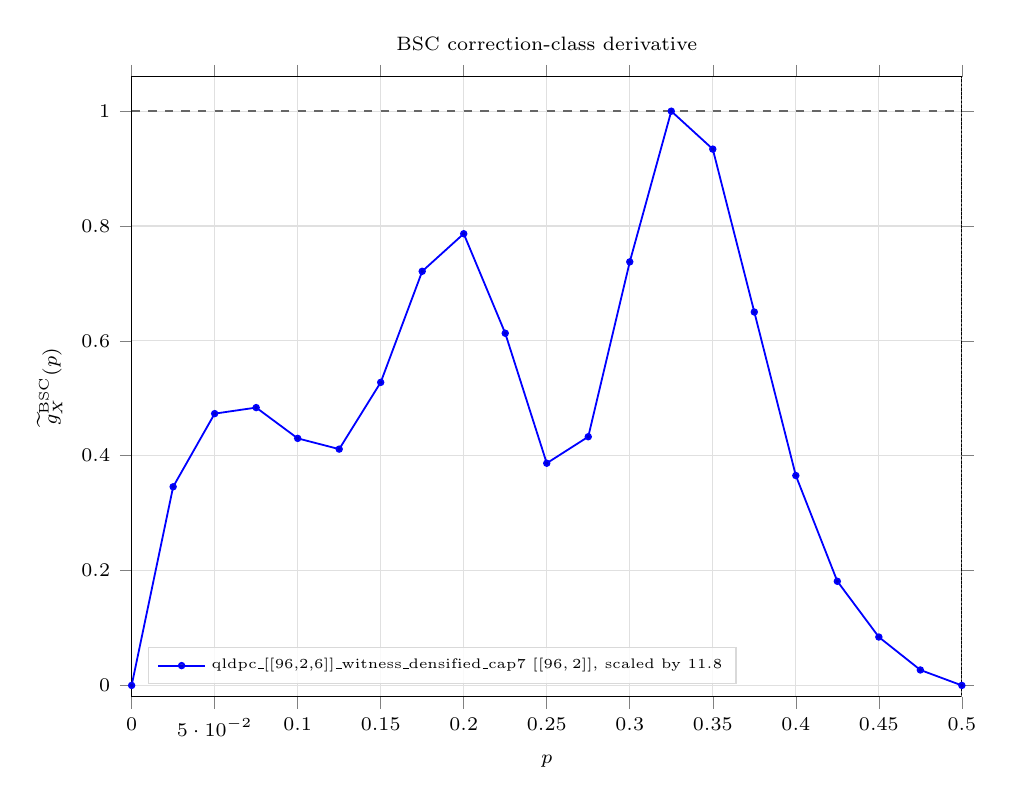
\begin{tikzpicture}
\begin{axis}[
  name=scaledBSCGEXITQldpc9626WitnessDensifiedCap7Axis,
  width=\linewidth,
  height=0.78\linewidth,
  title={BSC correction-class derivative},
  title style={font=\scriptsize},
  xlabel={$p$},
  ylabel={$\widetilde g_X^{\rm BSC}(p)$},
  xmin=0, xmax=0.5,
  ymin=-0.02, ymax=1.06,
  grid=both,
  major grid style={black!12},
  minor grid style={black!6},
  tick align=outside,
  tick label style={font=\scriptsize},
  label style={font=\scriptsize},
  legend cell align={left},
  legend style={draw=black!15, fill=white, fill opacity=0.82, text opacity=1, at={(0.02,0.02)}, anchor=south west, font=\tiny},
]
\addplot[black!60, densely dotted, line width=0.55pt, forget plot] coordinates {(0.5,-0.02) (0.5,1.06)};
\addplot[black!60, dashed, line width=0.55pt, forget plot] coordinates {(0,1) (0.5,1)};
\addplot+[color=blue, mark=*, mark size=1.0pt, line width=0.65pt]
coordinates {(0,0) (0.025,0.345930076401) (0.05,0.473309522882) (0.075,0.483819436139) (0.1,0.430227358217) (0.125,0.411484828686) (0.15,0.527760600658) (0.175,0.721182245675) (0.2,0.786594428573) (0.225,0.613299806655) (0.25,0.38692586579) (0.275,0.433086612819) (0.3,0.737594433274) (0.325,1) (0.35,0.933931208001) (0.375,0.650284631856) (0.4,0.365499637565) (0.425,0.181336634433) (0.45,0.0842975595535) (0.475,0.0268994621673) (0.5,0)};
\addlegendentry{qldpc\_[[96,2,6]]\_witness\_densified\_cap7 $[[96,2]]$, scaled by $11.8$}
\end{axis}
\end{tikzpicture}
